%!TEX root = /Users/velrok/Dropbox/TheoInf Seminar/Ausarbeitung/Main.tex


\section{Basic modal logic ($K$)} % (fold)
\label{sec:basic_modal_logic}

\subsection{Syntax} % (fold)
\label{sec:syntax}
Die Syntax der Modal Logik ist wie die der Aussagenlogik mit den Erweiterungen $\square$ und $\Diamond$. 
Wie die Negation sind diese unär, das heißt sie beziehen sich nur auf die ihr folgende Formel. Im Folgenden werden die Zeichen $p, q, r, p_3$ für atomare Formeln verwendet.\cite[S.307f]{huth2004logic}\\
\\
Die folgende BNF (Backus Naur Form) beschreibt die Syntax der möglichen multi modal Formeln $\phi$.

\begin{equation}
	\phi ::= \bot|\top|p|(\neg\phi)|(\phi\wedge\phi)|(\phi\vee\phi)|(\phi\rightarrow\phi)|
	(\phi\leftrightarrow\phi)|(\square\phi)|(\Diamond\phi)
\end{equation}

\begin{figure}[ht]
	\begin{center}
  	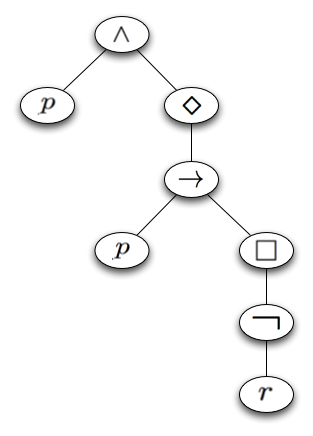
\includegraphics[width=0.4\textwidth]{./Images/mmFormel01.png}
		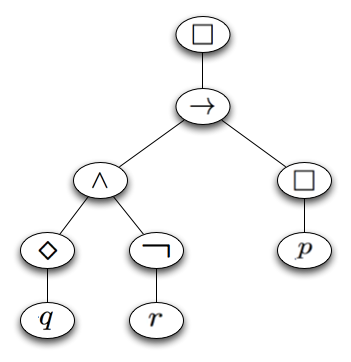
\includegraphics[width=0.4\textwidth]{./Images/mmFormel02.png}
  	\caption{Parse-Tree für $(p \wedge \Diamond(p \rightarrow \square \neg r))$ und 
		$\square((\Diamond q \wedge \neg r) \rightarrow \square p )$}
		\label{fig:mmFormel01}
	\end{center}
\end{figure}


Die Formeln $(p \wedge \Diamond(p \rightarrow \square \neg r))$ und 
$\square((\Diamond q \wedge \neg r) \rightarrow \square p )$ sind Beispiele für syntaktisch korrekte Multi-Modal-Logik Formeln. Ihre Parse-Trees sind abgebildet in Abbildung~\ref{fig:mmFormel01}.\\
\\
Wie auch bei der Aussagenlogik binden die unären Operatoren stärker als die Binären.
Sodass unnötige Klammern weggelassen werden können um die Leserlichkeit zu verbessern.\\
\\
Die folgende Liste sortieren die Operatoren nach ihrer Bindungsstärke. Beginnend mit den am stärksten bindenden.\\
\begin{itemize}
	\item $\neg, \square, \Diamond$
	\item $\wedge, \vee$
	\item $\rightarrow, \leftrightarrow$
\end{itemize}

Im allgemeinen werden die Symbole $\square$ und $\Diamond$ als Box und Raute gelesen. 
Spezifiziert man eine konkrete Logik so werden diese entsprechend ihrer interpretation gelesen. In der Logik für Notwendigkeit wird $\square$ als notwendig und $\Diamond$ als möglich gelesen. In Logik für über das Wissen eines Agenten Q, wird $\square$ als Q weis und $\Diamond$ als soweit Q weis, gelesen.


% section syntax (end)

\subsection{Semantik} % (fold)
\label{sec:semantik}

Dieses Kapitel beschreibt die Semantik von Modal-Logik-Aussagen. 
Die Semantik wird dabei formal beschrieben. Die grundlegende Frage ist wann evaluiert eine Modal-Logik-Formel zu \emph{wahr} bzw. \emph{falsch}.

Zur Erinnerung: In der Aussagenlogik ist eine Interpretation eine mögliche Belegung der Variablen mit den Wahrheitswerten \emph{Wahr} oder \emph{Falsch}. Dabei muss jeder der Variablen einen dieser Werte annehmen. Die Formel $a \wedge b$ hat $2_2 = 4$ mögliche Interpretationen. 
\begin{figure}[ht]
	\begin{center}
		\begin{tabular}{cccc}
		\hline
		a & b & $a \wedge b$\\
		\hline
		1 & 1 & Wahr\\
		\hline
		1 & 0 & Falsch\\
		\hline
		0 & 1 & Falsch\\
		\hline
		0 & 0 & Falsch\\
		\hline
		\end{tabular}
		\caption{Alle möglichen Interpretationen der Aussagenlogik-Formel $a \wedge b$}
		\label{tab:AussagenlogikInterpretation}
	\end{center}
\end{figure}
Siehe Abbildung~\ref{tab:AussagenlogikInterpretation}
\cite{hunter1973metalogic}% wikipedia: Was ist eine Interpretation http://en.wikipedia.org/wiki/First-order_logic#Evaluation_of_truth_values

Die Modal-Logik erfordert ein komplexeres Model für die Auswertung von Formeln, da verschiedene Arten von Wahr modelliert werden können.\cite[S.308f]{huth2004logic}

Ein Model in Modal-Logik wird deswegen durch eine Kripkestruktur beschrieben. 
Eine Kripkestruktur besteht aus einer Menge von Welten $W$, einer Relation $R:(WxW)$ auf diesen Welten, die angibt welche Welten $w'$ von einer Welt $w$ erreichbar sind und einer Label-Funktion $L: W \rightarrow P$. 
Die Label-Funktion weist jeder Welt $w$ eine Menge von Atomen $P$ zu und definiert damit die Wissensbasis. 

Nehmen wir an die Menge der Welten $W$ sei 
\begin{center}
	$\{ x_1, x_2, x_3, x_4, x_5, x_6 \}$
\end{center}
 
die Relation $R$ sei definiert als 
\begin{center}
	$\{(x_1, x_2), (x_1, x_3), (x_2, x_3), (x_3, x_2), (x_2, x_2), (x_4, x_5), (x_5, x_4), (x_5, x_6)\}$ 
\end{center}

und die Labelfunktion $L$ liefere,
\begin{center}
	\begin{tabular}{c|cccccc}
		$x$ & $x_1$ & $x_2$ & $x_3$ & $x_4$ & $x_5$ & $x_6$\\
		\hline
		$L(x)$ & $\{q\}$ & $\{p,q\}$ & $\{p\}$ & $\{q\}$ & $\{\}$ & $\{p\}$
	\end{tabular}
\end{center}

dann ist Abbildung~\ref{fig:mmKripke01} die graphische Darstellung der beschriebenen Kripke-Struktur.

\begin{figure}[ht]
	\begin{center}
  	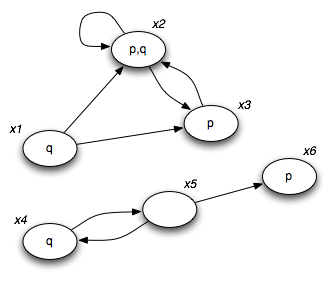
\includegraphics[width=0.65\textwidth]{./Images/Kripke01.png}
  	\caption{Beispiel einer Kripke-Struktur}
		\label{fig:mmKripke01}
	\end{center}
\end{figure}


Die Formeln \eqref{eqn:semanticTrue} bis \eqref{eqn:semanticLast} beschreiben formal unter welchen Gegebenheiten sich etwas folgern lässt.

\begin{align}
%	\begin{split}
	x &\vDash \top\label{eqn:semanticTrue}\\
	x &\nVDash \bot\label{eqn:semanticFalse}\\
	x &\vDash p\text{ gdw. }p \in L(x)\\
	x &\vDash \neg \phi\text{ gdw. }x \nVDash \phi\\
	x &\vDash \phi \wedge \psi\text{ gdw. }x \vDash \phi\text{ und } x \vDash \psi\\
	x &\vDash \phi \vee \psi\text{ gdw. }x \vDash \phi \text{, oder } x \vDash \psi\\
	x &\vDash \phi \rightarrow \psi\text{ gdw. }x \vDash \psi\text{, immer wenn gilt }x \vDash \phi\\
	x &\vDash \phi \leftrightarrow \psi\text{ gdw. }( x \vDash \phi\text{ gdw. }x \vDash \psi)\\
	x &\vDash \Box \psi \text{ gdw. }\forall y \in W \text{ gilt } R(x,y)\text{, und } y \vDash \psi\\
	x &\vDash \Diamond \psi\text{ gdw. }\exists y \in W \text{ sodass }R(x,y)\text{ und }y \vDash \psi\label{eqn:semanticLast}
%	\end{split}
\end{align}




% section semantik (end)

\subsection{Design neuer Logiken für eine bestimmte Modalität} % (fold)
\label{sub:design_neuer_logiken_fuer_eine_bestimmte_modalitaet}

\subsubsection{Ähnlichkeits Theorie}

% subsection design_neuer_logiken_für_eine_bestimmte_modalität (end)

% section basic_modal_logic (end)
